\documentclass[11pt]{scrartcl}

\usepackage[utf8]{inputenc}				% Umlaute
\usepackage[ngerman]{babel}				% Deutscher Text
\usepackage{chemmacros}					% Chem. Symbole
\usepackage{cite}						% Bibtex
\usepackage[onehalfspacing]{setspace}	% spacing
\usepackage{amsmath}					% more math
\usepackage{paralist}                   % compact lists
\usepackage{graphicx}					% figures
\usepackage{hyperref}					% links
\usepackage{verbatim}					% code
\usepackage{listings}					% code listings
\usepackage{ragged2e}					% justified text
\usepackage[numbers]{natbib}

\renewcommand{\bf}[1]{\textbf{#1}}
\renewcommand{\it}[1]{\textit{#1}}

\hypersetup{
    pdftitle={Bodenatmung im Nationalpark Hainich},
    pdfauthor={Jalali, Loos, Sichting},
    pdfsubject={Projekt zur Vorlesung Statistische Verfahren SoSe 2016},
    pdfkeywords={Statistik, Bodenatmung, Hainich, Projekt 9},
    bookmarksnumbered=true,     
    bookmarksopen=true,         
    bookmarksopenlevel=1,
    hidelinks,            
    pdfstartview=Fit,           
    pdfpagemode=UseOutlines
}

%listings
\lstset{
	language=R,
	basicstyle=\small\ttfamily,
	tabsize=4,
	breaklines=true,
	numbers=left,
	extendedchars=true, %utf-8	
	numberstyle=\footnotesize\color[RGB]{128,128,128},
	commentstyle=\color[RGB]{27,116,41},
	stringstyle=\color[RGB]{186,58,38},
	keywordstyle=\color[RGB]{33,73,114}
}


\title{Bodenatmung im Nationalpark Hainich}
\subtitle{Erstellung eines statistischen Modells und Diskussion von Fehlentscheidungen im Rahmen der Variablenselektion}
\author{Claudia Sichting (161915) \and Daniel Loos (161586) \and Roya Jalali (159939)}

\begin{document}
	\maketitle
	
	\centering{\Large{
				PROJEKTARBEIT\\
				im Rahmen des Moduls \it{Statistische Verfahren}\\
				Dr. Jens Schumacher
				\\
				an der Friedrich-Schiller-Universität Jena
			}}
	
	\begin{abstract}
		Die Freisetzung von \ch{CO2} in die Atmosphäre ist ein fundamentaler Bestandteil von Modellen zur Berechnung klimatischer Phänomene.
		Die \it{Bodenatmung} ist hierbei der dominierende Prozess auf Landgebieten.
		Zur Modellierung dieses Prozesses wurde im Nationalpark Hainich Messdaten im Einfluss von 32 Variablen erhoben.
		Daraus wird nun ein statistisches Modell erstellt.
		Bei der Variablenselektion können statistische Unsicherheiten zu Fehlern führen.
		Dies wird im folgendem diskutiert.
	\end{abstract}
	
	\justify
	
	\newpage
	\tableofcontents
	\newpage
	
	\section{Einleitung}
\label{sec-intro}

\subsection{Bodenatmung als geophysikalischer Prozess}
\cite{foo}

\subsection{Statistische Grundlagen}

\subsubsection{Fehlermaße}
RSS (\it{Residual sum of Suqres}).
SPSE ist der summierte quadratische Fehler zwischen Modellvorhersage und Messwert auf unabhängigen Testdaten:
\begin{equation}
	\widehat{SPSE} = \sum_{i=1}^n (y_i - \vec{\beta} * x_i^T )^2
\end{equation}
Das Modell wurde vorher mit anderen Trainingsdaten erstellt.

\subsubsection{Korrelation}
Unter \it{Korrelation} versteht man die „Wechselbeziehung“ zweier Zufallsgrößen.
Dieser Zusammenhang kann entweder \it{linear} (Korrelationskoeffizient nach Pearson) oder lediglich \it{monoton} sein.
Ist eine Korrelation nicht gegeben, so scheint die Zufallsgröße als ungeeigneter Prädiktor für die jeweils andere Variable.
Kausale Beziehungen erfordern Korrelation.
\\
Der \it{lineare, empirische Korrelationskoeffizient nach Person} zwischen den Variablen $X$ und $Y$ wird definiert durch:
\begin{equation}
	Kor_e(x,y) := \varrho_e(x,y) := r_{xy} := \frac{
		\sum_{i=1}^n(x_i-\bar x)(y_i-\bar y)
	}{
	\sqrt{
		\sum_{i=1}^n(x_i-\bar x)^2\cdot
		\sum_{i=1}^n(y_i-\bar y)^2
	}
	}
\end{equation}
mit den empirischen Mittelwert $\bar x$ aus $n$ Messwerten von $X$.
Möchte man lediglich ein \it{lineares} Modell erstellen, so ist die Pearson-Korrelation zu wählen.
\\
Eine allgemeinere Beschreibung der Korrelation ist die nach \it{Spearsman}, welche auf Ranglisten beruht:\\
\begin{align}
	r_s &= \frac{\sum_{i}(rg(x_i)-\overline{rg}_x)(rg(y_i)-\overline{rg}_y)} {\sqrt{\sum_{i}(rg(x_i)-\overline{rg}_x) ^2}\sqrt{\sum_{i}(rg(y_i)-\overline{rg}_y)^2}}\\
	&= \frac { \frac{1}{n} \sum_{i}(rg(x_{i})  rg(y_{i})) - \overline{rg_x rg_y}  }{s_{rg_x} s_{rg_y}} \\
	&= \frac {{Cov}(rg_{x},rg_{y} )} { s_{rg_x} s_{rg_y} }
\end{align}
Somit lassen sich auch nicht-lineare Korrelationen in Datensätzen erkennen.
Insbesondere im Betrachtung des exponentiellem Verhaltens in Abhängigkeit von der Temperatur ist diese Art der Korrelation wichtig.
Zur Berechnung des Anteils an der \it{erklärten} Varianz in linearen Modellen allerdings kann diese Variante nicht verwendet werden.

\subsubsection{Informationskriterien}

Je mehr Variablen für ein Modell in Betracht gezogen werden, um so komplexer wird es. Meist wünscht man sich aber ein einfaches Modell, dass mit möglichst wenigen Variablen sehr gute Vorhersagen treffen kann. Mit verschiedenen Informationskriterien kann man nach Variablen mit der minimale Varianz der Residuen suchen. Das \emph{Bayessches Informationskriterium (BIC)}\footnotetext[1]{Schwarz-Bayes Criterion (SBC))} ist im Vergleich zu \emph{Akaikes Informationskriterium} abhängig von der Stichprobengröße.

$$\displaystyle AIC_{\ell }=-2\ell (\mathbf {\hat {\theta }} )+2k$$

$$\displaystyle BIC_{\ell }=-2\ell (\mathbf {\hat {\theta }} )+\log(n)k$$

Dies machen wir uns bei unseren Testdaten nützlich, da unsere Stichprobe recht klein ist. Zusätzlich betrachten wir noch das \emph{korrigierte Bestimmtheitsmaß  $\bar{R^2}$ (adjr2; engl. \it{adjusted r-squared})}. Es ist im Vergleich zum Bestimmtheitsmaß $R^2$ angepasst an die Anzahl der Variablen im Modell. Es steigt nur an, wenn die Variable das Modell stärker verbessert als der Zufall, ansonsten sinkt es.

$$\bar R^2 = 1- (1-R^2) \frac{n-1}{n-p-1} = R^2 - (1-R^2) \frac{p}{n-p-1}$$

(33 Variablen mit je 38 Messungen, von denen einige wegfallen, weil sie nicht normalverteilt sind.)
Adjusted r-squared
BIC/AIC

\subsubsection{Test auf Vorliegen einer Normalverteilung}

Der \emph{Shapiro-Wilk-Test} ist ein statistischer Test zur Überprüfung der Hypothese, ob Variablen normalverteilt sind. Wenn bei dem Test die p-Value großer als 0.05 ist, dann ist die Variable normalverteilt.
dieses Test ist benutzbar wenn die Anzahl der Variablen zwischen 3 und 5000 ist. Somit ist es geeignet für unsere Variablen. Der Test basiert auf der Teststatistik W, der den graphischen Überprüfungen (zum Beispiel QQ-Plot) einen Wert zuweist.

$$\textit{W} = {{b^2}\over {(n-1)s^2}}$$

\cite{2012shapiro}

Mit $b^2$ als quadrierte Steigung der Regressionsgeraden im QQ-Plot.

Zur Überprüfung der Nullhypothese fasst das Shapiro-Wilk-Testverfahren die graphischen Informationen in einer Kennzahl zusammen, die einer Analyse mittels Normalwahrscheinlichkeitsplot entspringen würden. Diese Kennzahl, die Teststatistik W, drückt das Verhältnis zweier Varianz-Schätzer zueinander aus.


Der Ausdruck im Zähler der Teststatistik schätzt die Varianz einer Stichprobe, die aus einer normalverteilten Grundgesamtheit stammt. Die Teststatistik vergleicht dann diese unter der Nullhypothese „erwartete“ Varianz mit der tatsächlichen Varianz der Stichprobe, deren Schätzer im Nenner der Teststatistik zu finden ist. 

\subsubsection{F-Test in geschachtelten Modellen}
Der \it{F-Test} überprüft, ob zwei verschachtelte Modelle mit den Featuremengen $M_1 \subseteq M_2$ sich signifikant unterscheiden.
Hierbei wird auf den gleichen Testdaten evaluiert.
Unter Annahme der Nullhypothese ist die Test-Statistik F-verteilt und abhängig von den Freiheitsgraden (Anzahl der Features im Modell).
Mit der Nullhypothese wird überprüft, ob die hinzugefügten Features des erweiterten Modells statistisch irrelevant sind ($H_0: \beta_i = 0$).

Die F-Statistik wird gebildet durch:
\begin{equation}
	F=\frac{\frac{RSS_1-RSS_2}{p_2-p_1}}{\frac{RSS_2}{n-p_2}}
\end{equation}
mit den quadrierten Residuen $RSS$, den Freiheitsgraden $p_i$ in den Modellen $M_1$ und das um weitere Feature erweiterte Modell $M_2$.
Ist der F-Wert je nach Signifikanzniveau hinreichend groß, kann die Nullhypothese abgelehnt werden:
Das erweiterte Modell beschreibt die Daten nun signifikant genauer.
Der Fehler $RSS$ wird so stark verringert, dass es auch eine Erhöhung der Freiheitsgrade rechtfertigt. 
\\
Die R-Funktion \lstinline|anova(model1, model2)| führt derartige Tests durch. Ist der p-Value (in R \lstinline|F Pr(>F)|) kleiner als das Signifikanzniveau, so wird im Rahmen der Variablenselektion das erweiterte Modell favorisiert.

	\newpage
	\section{Erstellung eines Modells zur Bodenatmung}
\label{sec-model}

Der Datensatz enthält sehr viele Features im Vergleich zur Anzahl an Messungen.
Der Suchraum der Variablenselektion wäre viel zu groß und muss demnach verkleinert werden.
Außerdem ist eine Schätzung von so vielen Parametern mit vergleichsweise wenigen Messungen auch statistisch zu ungenau.

\subsection{Test auf Vorliegen einer Normalverteilung}

Es werden nur normalverteilte (\it{Shapiro-Wilk}) und stark korrelierende (\it{Pearson}) Variablen in Betracht gezogen. Um \it{Pearson} als Korrelationskoeffizienten nutzen zu können, müssen die Messungen der Variablen normalverteilt sein. Um dies zu testen nutzen wir den \it{Shapiro-Wilk-Test}. Wenn der \it{p-Value} des \it{Shapiro-Wilk-Tests} größer als das Signifikanzniveau $\alpha=0.05$ ist, dann ist die Variable normalverteilt. Wie in Abbildung \ref{fig:shapiro} zu sehen ist, sind nur 14 der insgesamt 33 Variablen normalverteilt.

\begin{figure}[ht]
	\centering
	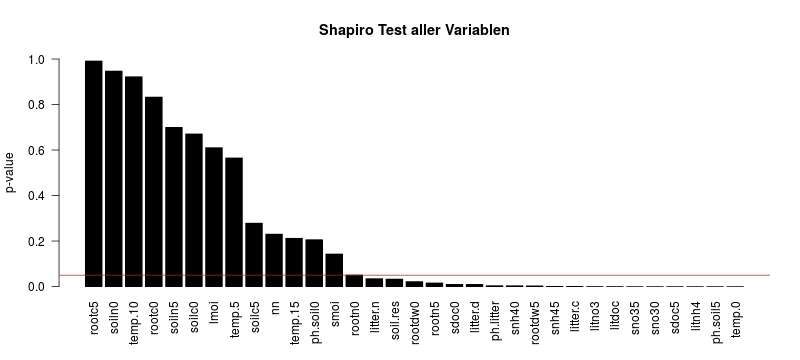
\includegraphics[width=\textwidth]{fig/model/normalverteilung-shapiro.png}
	\caption{\bf{P-Value des Shapiro-Wilk-Tests aller Variablen.}}
	\label{fig:shapiro}
\end{figure}

\subsection{Korrelationsanalyse}

Aus den normalverteilten Variablen werden die am stärksten korrelierenden Variablen ausgewählt (siehe Abbildung \ref{fig:pearson}). 

\begin{figure}
	\centering
	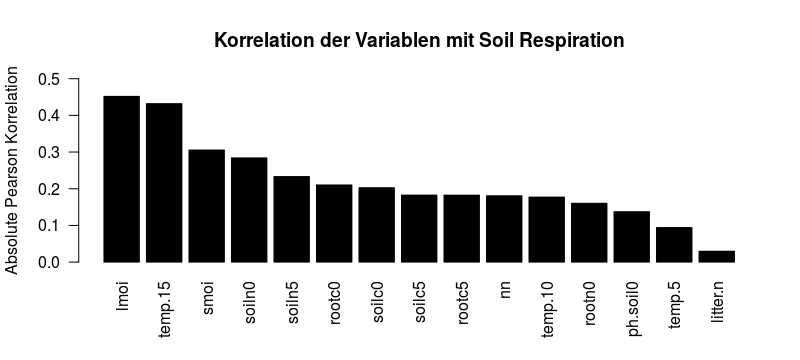
\includegraphics[width=\textwidth]{fig/model/correlation-pearson-normal.png}
	\caption{\bf{Pearson-Korrelation} der normalverteilten Einflussgrößen (\it{p-Value} $> 0.32$) mit der Bodenatmung.}
    \label{fig:pearson}
\end{figure}

\begin{compactitem}
\item
  \emph{lmoi} relative Feuchte der Streuschicht (litter moisture)
\item
  \emph{temp15} Bodentemperatur in 15 cm Tiefe
\item
  \emph{smoi} relative Bodenfeuchte (soil moisture)
\end{compactitem}

\subsection{Transformationen}

Lineare Modelle erfordern lineare Korrelationen.
Bei nicht linearen Korrelationen kann eine Linkfunktion als Transformation der Zufallsgröße verwendet werden, um die gewählte Messgröße zu linearisieren.
Soe \it{et. al.} verwendeten eine derartige Transformation vor allem für die Temperatur, da die Reaktionsgeschwindigkeit einer Reaktion exponentiell und nicht linear in Abhänigkeit der Temperatur verläuft.
Unsere Datenlage allerdings konnte die Notwendigkeit einer solchen Transformation nicht bestätigen (Vgl. Abbildung \ref{fig:temp}).
Eine hohe \it{Pearson}-Korelation bestätigte den Verdacht.
\begin{figure}
	\centering
	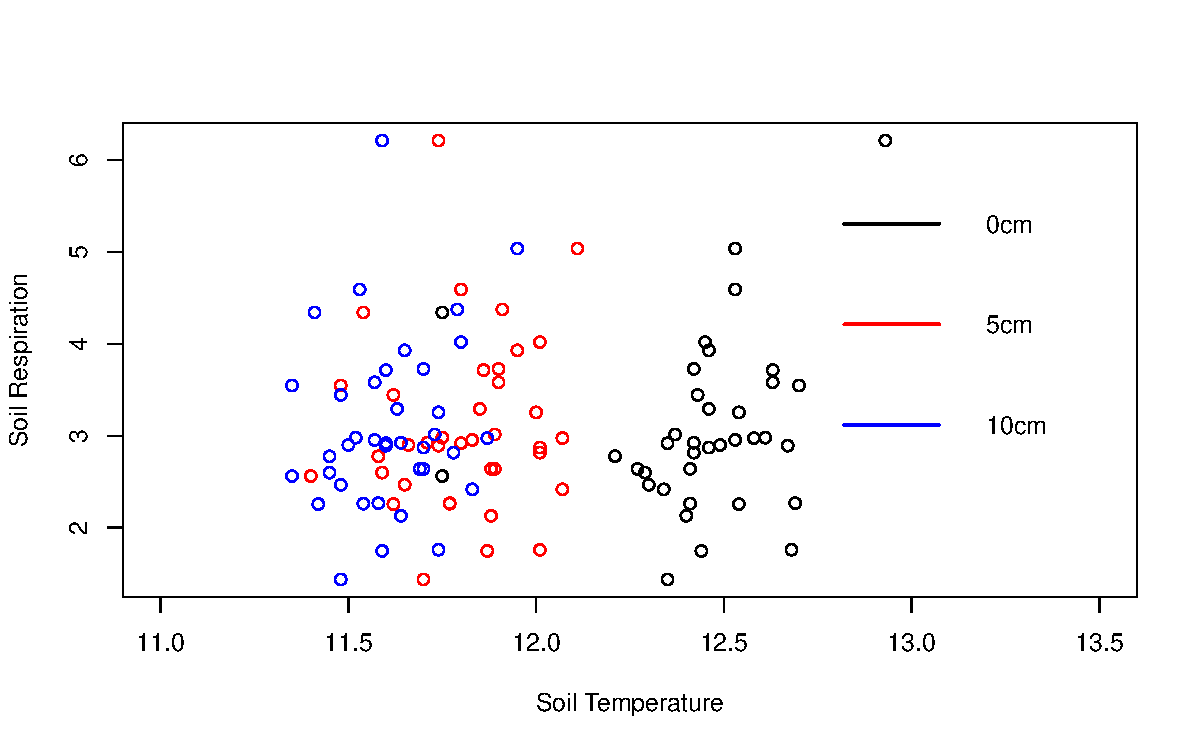
\includegraphics[width=\textwidth]{fig/model/temp-vs-resp.pdf}
	\caption{\bf{Bodenatmung in Abhänigkeit von der Temperatur.}
		 Es ist keine nichtlineare Korrelation der beiden Größen ersichtlich. }
	\label{fig:temp}
\end{figure}
Transformationen bringen keine deutlichen Verbesserungen der Variablen. 
Für diese Analyse wurde außerdem ein Scatterplot genutzt (Abbildung im Anhang).


\subsection{Variablenselektion}

Mit Hilfe des R-Pakets \emph{leaps} wird das Modell mit dem geringsten Wert des \emph{Bayesschem Informationskriteriums (BIC)} ausgewählt, welches das Kriterium der Modellqualität erfüllt.
In Abbildung \ref{fig:bic} sieht man, dass ein Hinzufügen der Variable $soiln0$ den BIC-Wert nur erhöhen würde.

\begin{figure}[ht]
	\centering
	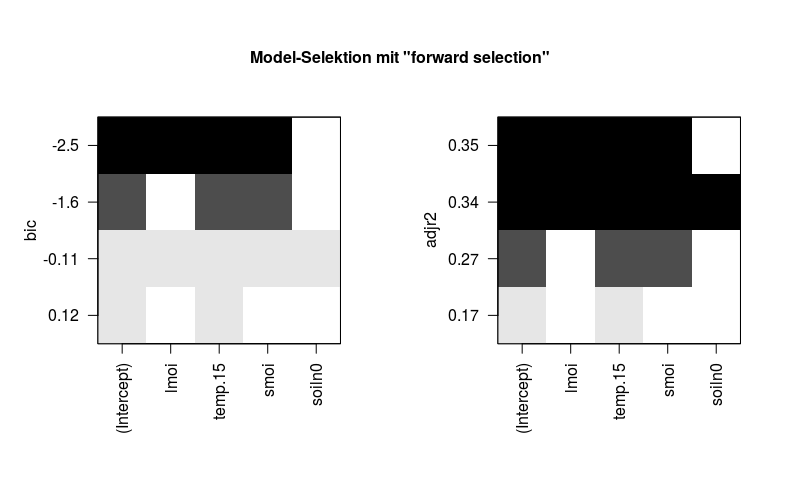
\includegraphics[width=\textwidth]{fig/model/variablenselektion-bic-adjr2.png}
	\caption{\bf{Variablenselektion mittels Bayesschem Informationskriterium (bic) und korrigiertes Bestimmtheitsmaß $\bar{R^2}$ (adjr22)}. Im linken Bild sieht man die Variablenselektion anhand des \emph{Bayesschem Informationskriteriums} und des \emph{korrigierte Bestimmtheitsmaßes}, die beide das Modell mit den ersten drei Variablen (\emph{lmoi, temp.15, smoi}) bevorzugt.}
    \label{fig:bic}
\end{figure}

\subsection{Ergebnis}
Bezüglich der Voraussetzungen der Normalverteilung, der Korrelation und des BICs wurde folgendes Modell zur Beschreibung der Bodenatmung ausgewählt:
$$soil.res = \vec{\beta} * (1,lmoi,temp15,smoi)^\text{T}$$

\subsection{Umsetzung mit R}

\begin{lstlisting}
# Test auf Normalverteilung
hainich.shapiro <- mapply(function(x) shapiro.test(x)$p.value,hainich)
hainich.normal <- hainich[names(hainich.shapiro[hainich.shapiro > 0.032])]
# Korrelation mit Pearson
hainich.pear <- abs(cor(hainich.normal))["soil.res",-16]
\end{lstlisting}

	\newpage
	\section{Simulation}
In Kapitel \ref{sec-model} wurde folgendes Modell ausgewählt:
\begin{equation}
	soil.res = \vec{\beta} * (1,lmoi,temp15,smoi)^T
\end{equation}

\subsection{Vorgehensweise}
Die Daten wurden in 80\% zum Training und 20\% zum Testen aufgeteilt.
Anschließend wurde das "wahre" Modell um jeweils ein weiteres Feature erweitert.
Das erweiterte Modell $soil.res = \vec{\beta} * (1,lmoi,temp15,smoi,x)^T$ wurde mittels ANOVA mit dem "wahren" Modell verglichen.
In R berechnete die Funktion \lstinline|anova(realModel, nxtModel)$F[2]| den jeweiligen F-Wert.
Wichtig hierbei war, dass beide Modelle auf den selben Trainingsdaten erstellt wurden und es sich um \it{verschachtelte} Featuremengen handelte.
Die Partitionierung der Daten erfolgte sowohl mittels Kreuzvalidierung als auch mit einem Monte-Carlo-Ansatz.
Bei der 4-fachen Kreuzvalidierung wurden die Daten in vier möglichst gleich großen Partitionen aufgeteilt.
Eine Partition wurde zum Testen des Reproduktionsfehlers verwendet, die Anderen zum Training.
Beim Monte-Carlo-Ansatz wurden 100 mal zufällig 20\% der Daten zum Testen ausgewählt.
Dadurch kann die Wahrscheinlichkeit der Fehlentscheidungen im Bezug auf die Nullhypothese besser geschätzt werden.
Die Ermittlung des Reproduktionsfehlers $\widehat{SPSE}$ erfolgte mittels unabhängigen Testdaten.
Um zu überprüfen, ob sich das Modell überhaupt verbessert hat, wurde die Differenz $\Delta \widehat{SPSE}$ im Bezug auf das Ausgangsmodell berechnet.

\subsection{Auswertung}
\begin{figure}[htbp]
	\centering
	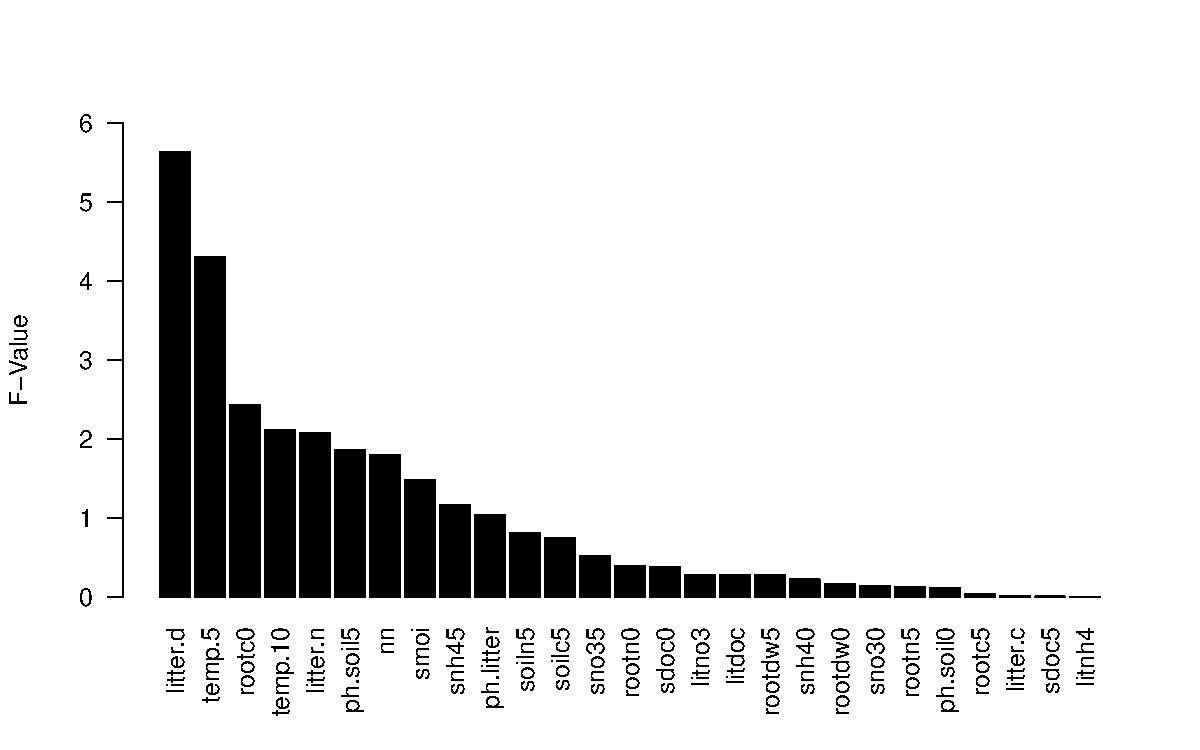
\includegraphics[width=\textwidth]{fig/simul/simul-f.pdf}
	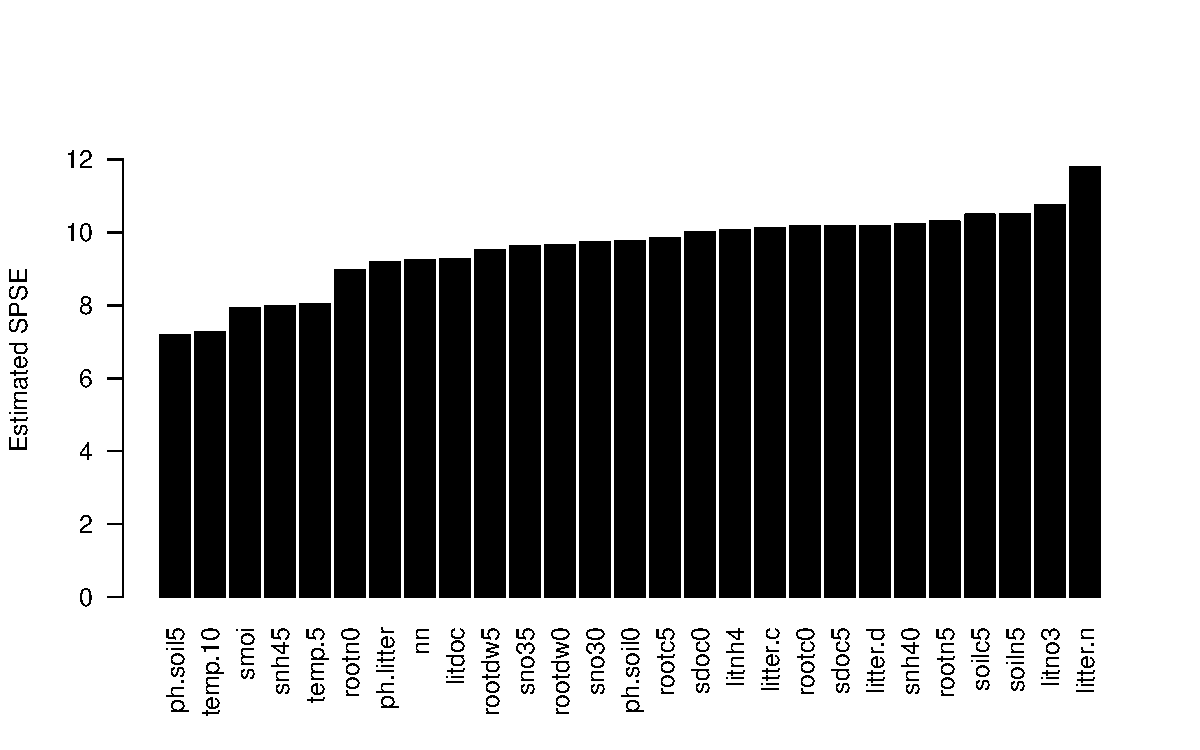
\includegraphics[width=\textwidth]{fig/simul/simul-spse.pdf}
	\caption{\bf{Beispiel einer Simulation.} 
		Das in Kapitel \ref{sec-model} erstellte "wahre" Modell wurde um jeweils ein Feature erweitert.
		Dargestellt ist der Fehler \bf{SPSE} und der zugehörige \bf{F-Wert} in Abhänigkeit von der gewählten zusätzlichen Variable in der ersten Runde der Kreuzvalidierung.
		Im Verlaufe der Variablenselektion wird das Modell mit dem höchsten F-Wert gewählt.
		Dies ist allerdings selten das Modell mit dem geringsten Fehler.
	}
	\label{fig-simul-f-spse}
\end{figure}
In Abbildung \ref{fig-simul-f-spse} sind die F-Werte und Fehler bei der Reproduktion von unabhängigen Testdaten gezeigt.
Im Rahmen des Variablenselektionsverfahrens wird jeweils das Feature zum Modell hinzugenommen, welches um den größten F-Wert verfügt.
Im diesem Falle wäre das $litter.d$.
Betrachtet man allerdings den erwarteten Reproduktionsfehler $\widehat{SPSE}$, so führt das Hinzunehmen der Variable $ph.soil5$ zum Modell mit minimalen Fehlern.
Hier ist der F-Wert aber um $\approx 3,5$ geringer.
Die Nullhypothese wird hier fälschlicherweise abgelehnt und stattdessen $litter.d$ zum Modell hinzugenommen.
Auch kann es vorkommen, dass eine Zufallsvariable überwiegend Rauschen beinhaltet und sich das Modell dann durch hinzufügen ebendieser Variable lediglich verschlechtert (Vgl. Abb. \ref{fig-simul-delta-spse})
\\
Nach der Monte-Carlo-Simulation war das Modell mit dem geringsten $\widehat{SPSE}$ stets das Modell mit den 9. höchsten F-Wert.
Während der 200 Simulationen verblieb der Wert unverändert.
\\
\begin{figure}[htbp]
	\centering
	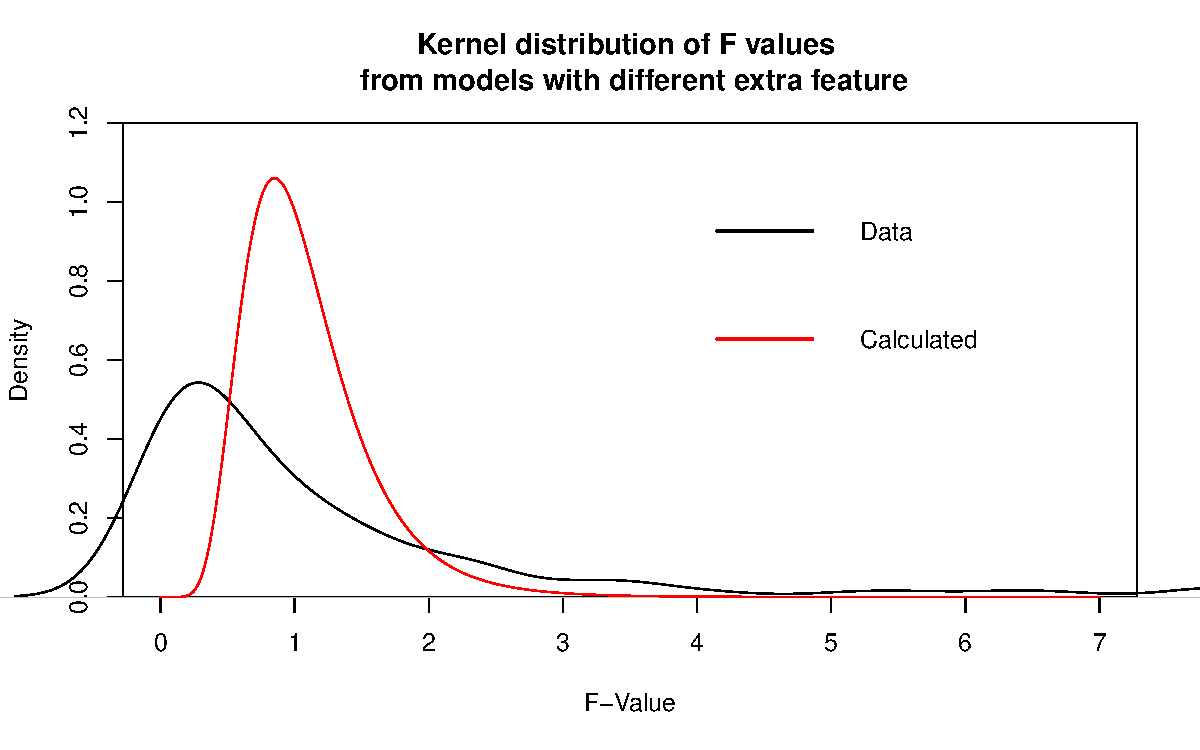
\includegraphics[width=\textwidth]{fig/simul/kernel.pdf}
	\caption{\bf{Approximierte Dichtefunktionen der F-Werte.} 
		Gezeigt ist die Kerneldichtefunktion der F-Werte der Simulationen und die berechnete F-Dichtefunktion mit den Freiheitsgraden der ANOVA-Tabelle unter Berücksichtigung der Nullhypothese.
		Der Unterschied der beiden Funktionen deutet auf fehlerhafte F-tests hin.
	}
	\label{fig-simul-kernel}
\end{figure}
Unter der Nullhypothese (Erweitertes Modell ist nicht besser als das "wahre" Modell) ist die F-Statistik eine F-verteilte Zufallsvariabel.
Die Dichtefunktion der Daten aus der Kreuzüberprüfung (approx. durch Kernel-Desity) ist nach Abb. \ref{fig-simul-kernel} mitunter stark abweichend.
Die Simulation möchte demnach das wahre Modell erweitern ($H_0$ wird abgelehnt).
Dies führt zu Overfitting, da das Modell bereits als wahr angenommen wurde und demnach keine weiteren Features hinzugefügt werden sollten.

\subsection{Diskussion}

\subsubsection{Mögliche Gründe}
Dies kann mehrere Gründe haben:
Gemessene Features müssen nicht zwangsläufig von der Bodenatmung statistisch abhängig sein.
Je geringer die Korrelation dieser beiden Zufallsvariablen, desto höher ist die Wahrscheinlichkeit, dass es sich nur um Rauschen handelt.
In diesem Fall sollte diese Variabel nicht zum Modell hinzugefügt werden.
Zufälligerweise kann dies aber auch zu hohen F-Werten führen, welches zu fehlerhaften Entscheidungen bei den Hypothesentests führt.
Ferner fordert der F-Test normalverteilte Variablen.
Folgt eine Messgröße nicht dieser Verteilung, ist der Test nicht aussagekräftig.
Auch eine nicht repräsentative Stichprobe fälscht das Ergebnis.
Uns lagen lediglich 38 Observationen vor; dies könnte zu gering sein.
Eine fehlerhafte Datenerhebung führt auch zu verfälschten Ergebnissen.
Letztendlich kann der F-Test auch nur zufällig richtig sein.
Ein geringer p-Value schließt keine Fehlentscheidungen aus; sie werden lediglich unwahrscheinlicher.

\subsubsection{Auswirkungen der Fehlentscheidungen}

\begin{figure}[htbp]
	\centering
	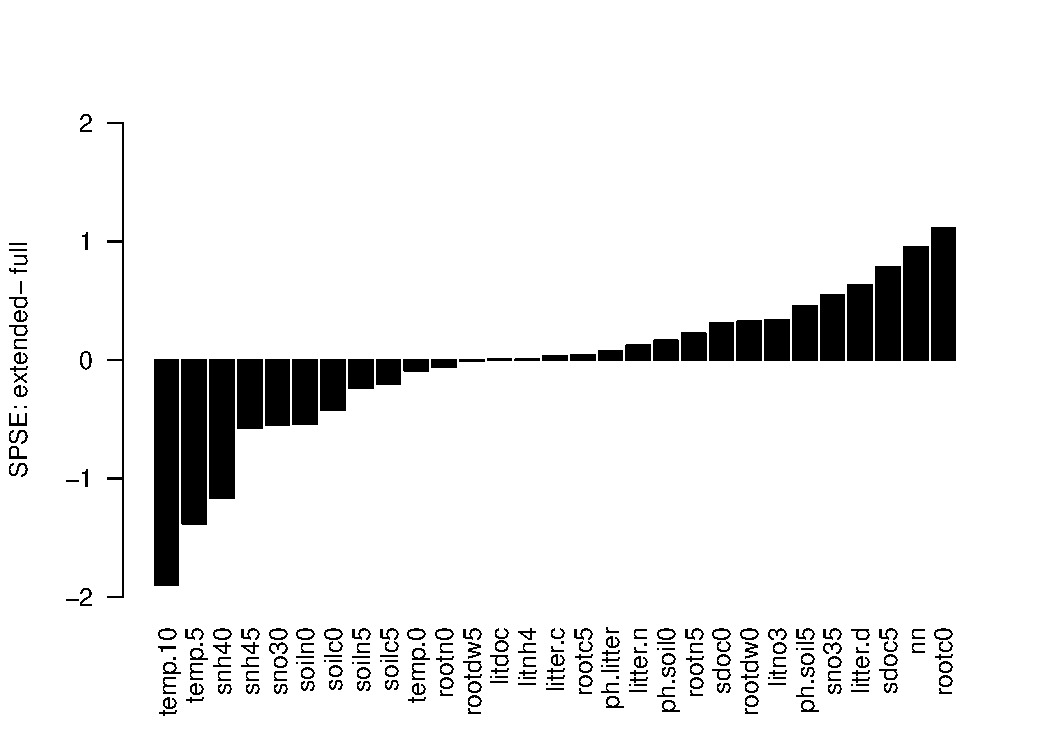
\includegraphics[width=\textwidth]{fig/simul/delta-spse.pdf}
	\caption{\bf{Verbesserung der Modelle.} 
		Dargestellt ist die Differenz $\Delta \widehat{SPSE}$ aus dem „wahren“ und dem erweiterten Modell.
		Positive Werte deuten darauf hin, dass die hinzugefügte Variable dem Modell lediglich Rauschen beifügt.
	}
	\label{fig-simul-delta-spse}
\end{figure}

	\newpage
	\section{Code}

\subsection{Korrelation}
\lstinputlisting{fig/code/hainich-correlation.r}

\subsubsection{Korrelation der Temperatur}
\lstinputlisting{fig/code/hainich-correlation-temp-resp.r}

\subsection{Variablenselektion}
\lstinputlisting{fig/code/hainich-variablenselektion.r}

\subsection{Simulation}
\subsubsection{Monte-Carlo}
\lstinputlisting{fig/code/hainich-f-simul-monte.r}
\subsubsection{Kreuzvalidierung}
\lstinputlisting{fig/code/hainich-f-simul-crossval.r}

	\bibliographystyle{unsrtnat}
    \bibliography{hainich}
	
\end{document}
